\chapter{OptimalSort}

\label{chap:OptimalSort}


OptimalSort is an online card sorting tool which is provided by the Optimal Workshop company. 
There are also tools for Tree Testing, First-click Testing, Online Surveys and Qualitative Research 
provided by them. 
OptimalSort is really intuitive to use for both the participants and the creator of the study. 
Unfortunately, there is a paywall for using all features of the tool, but also with the free plan the 
basic features of card sorting and analysis are available and it can easily keep up with all the other 
reviewed tools~\parencite{OptimalSort}.


\begin{figure}[h] 
\centering
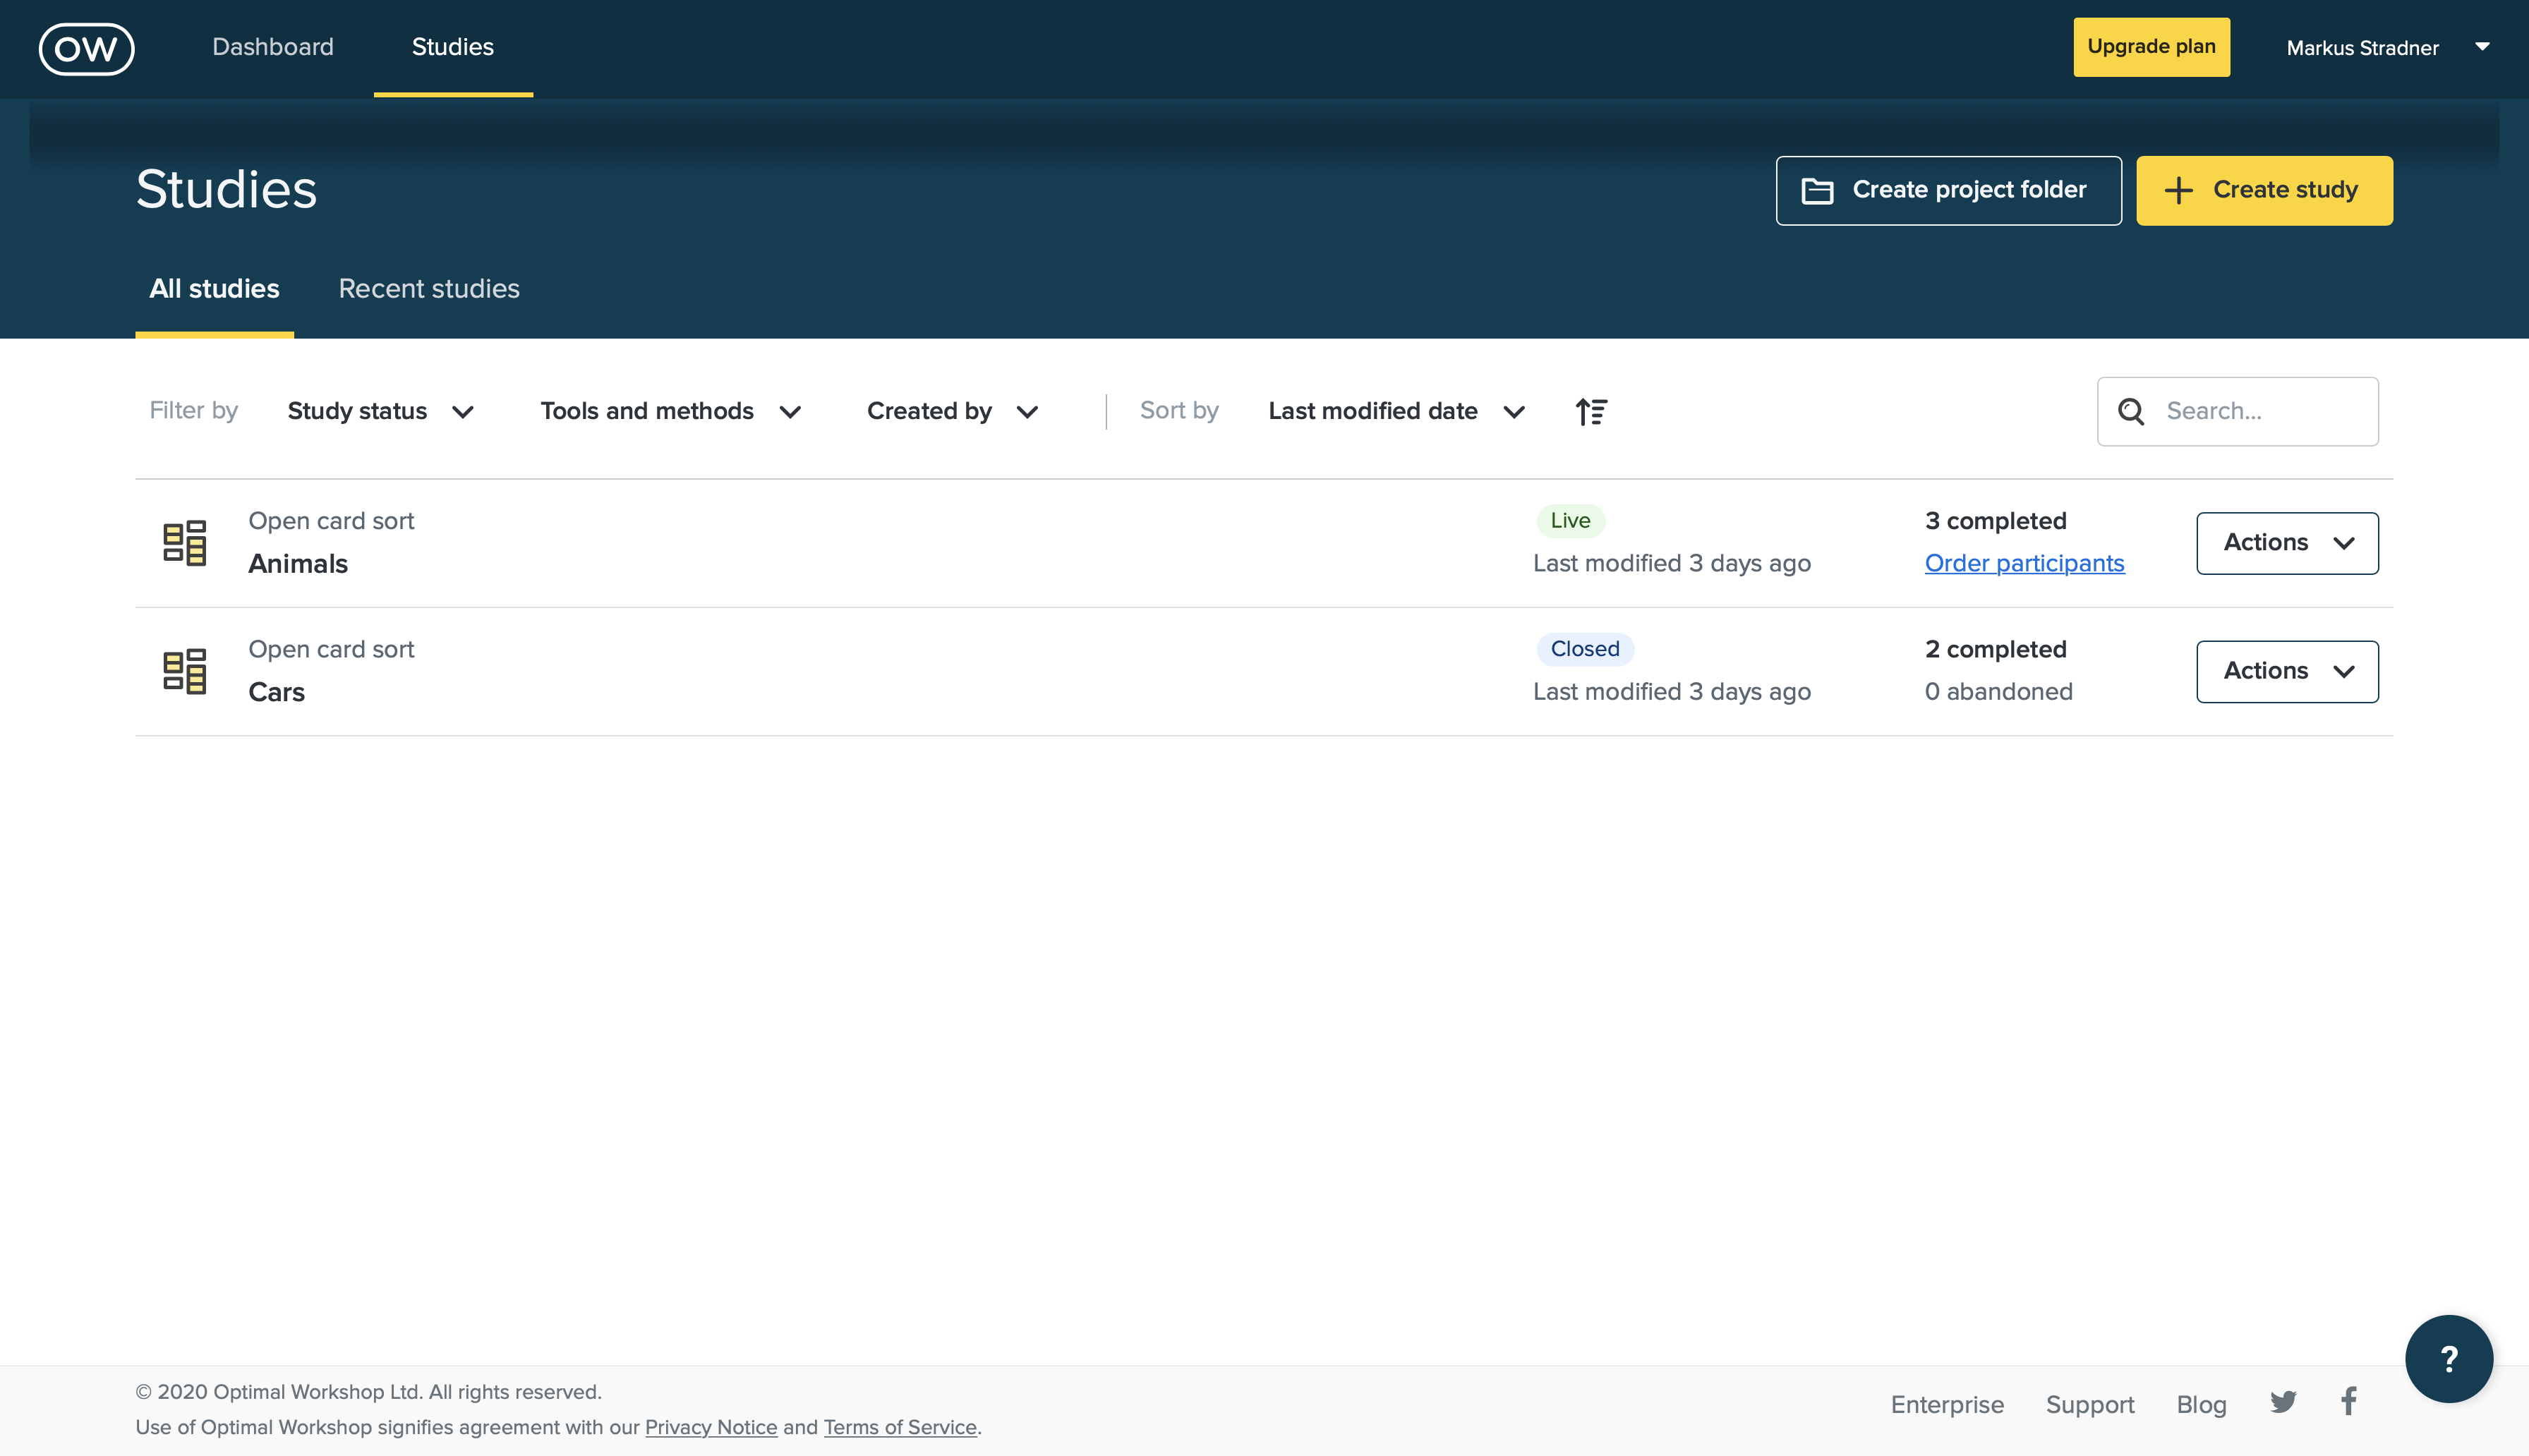
\includegraphics[keepaspectratio,width=\linewidth,height=\halfh]{images/optimalsort-studies.png}
\caption[OptimalSort Application] { This is the view of all studies in OptimalSort.
It shows you an overview of all your studies and in the dropdown button "Actions"
further actions can be performed.
\imgcredit{Screenshot was captured by Markus Stradner using
\textcite{OptimalSort} on Safari 14.0.1, 28.11.2020.} }
\label{fig:OptimalSort1}
\end{figure}


\section{Business Model}
As OptimalSort is provided by the Optimal Workshop company it is obvious that not all features 
of the tool are offered for free. 
For getting access to all features of all the tools of Optimal Workshop you have to upgrade 
your plan which is then \$166 per month. There is no opportunity to pay possibly less to use 
card sorting only. 

In the free version the number of cards is limited to thirty and the number of participants to ten.
Furthermore you are not allowed to define a closing rule, use password protection, reflect your 
brand in the study and add screening questions at the start of the study. 
Also for using the free version registration is required. There it is also offered to sign in 
with an existing Google account. All created studies and participations are saved to your 
account on their server. This also means that it doesn't matter which device you use.


\section{Card Sorting}
Setting up a card sorting with OptimalSort is quite comfortable. At the beginning you land on the 
dashboard, which is very well designed. On this page you can also do tutorials, watch demos and 
use the resource center, where you can access help, reading through the new features and also
give feedback.

The study creation process is very straight forward. They offer an import function for cards and
categories (closed card sorting) with a spreadsheet, pre-defined editable welcome and thank you
messages, a preview mode and automatic saving. Moreover you can edit the link of the study
yourself. 

In the paid version you can additionally create a questionnaire, define a closing rule, use
password protection and also show your logo in the study.

Once the study has been launched it is possible to share the study with other people via a link. 
Also when clicking on such a link and participating in a card sorting all the steps are 
very intuitive. At first the welcome screen with a short welcome message is shown. After clicking 
continue the instructions with 4 steps help you to get used to the sorting. 

\begin{figure}[h] 
\centering
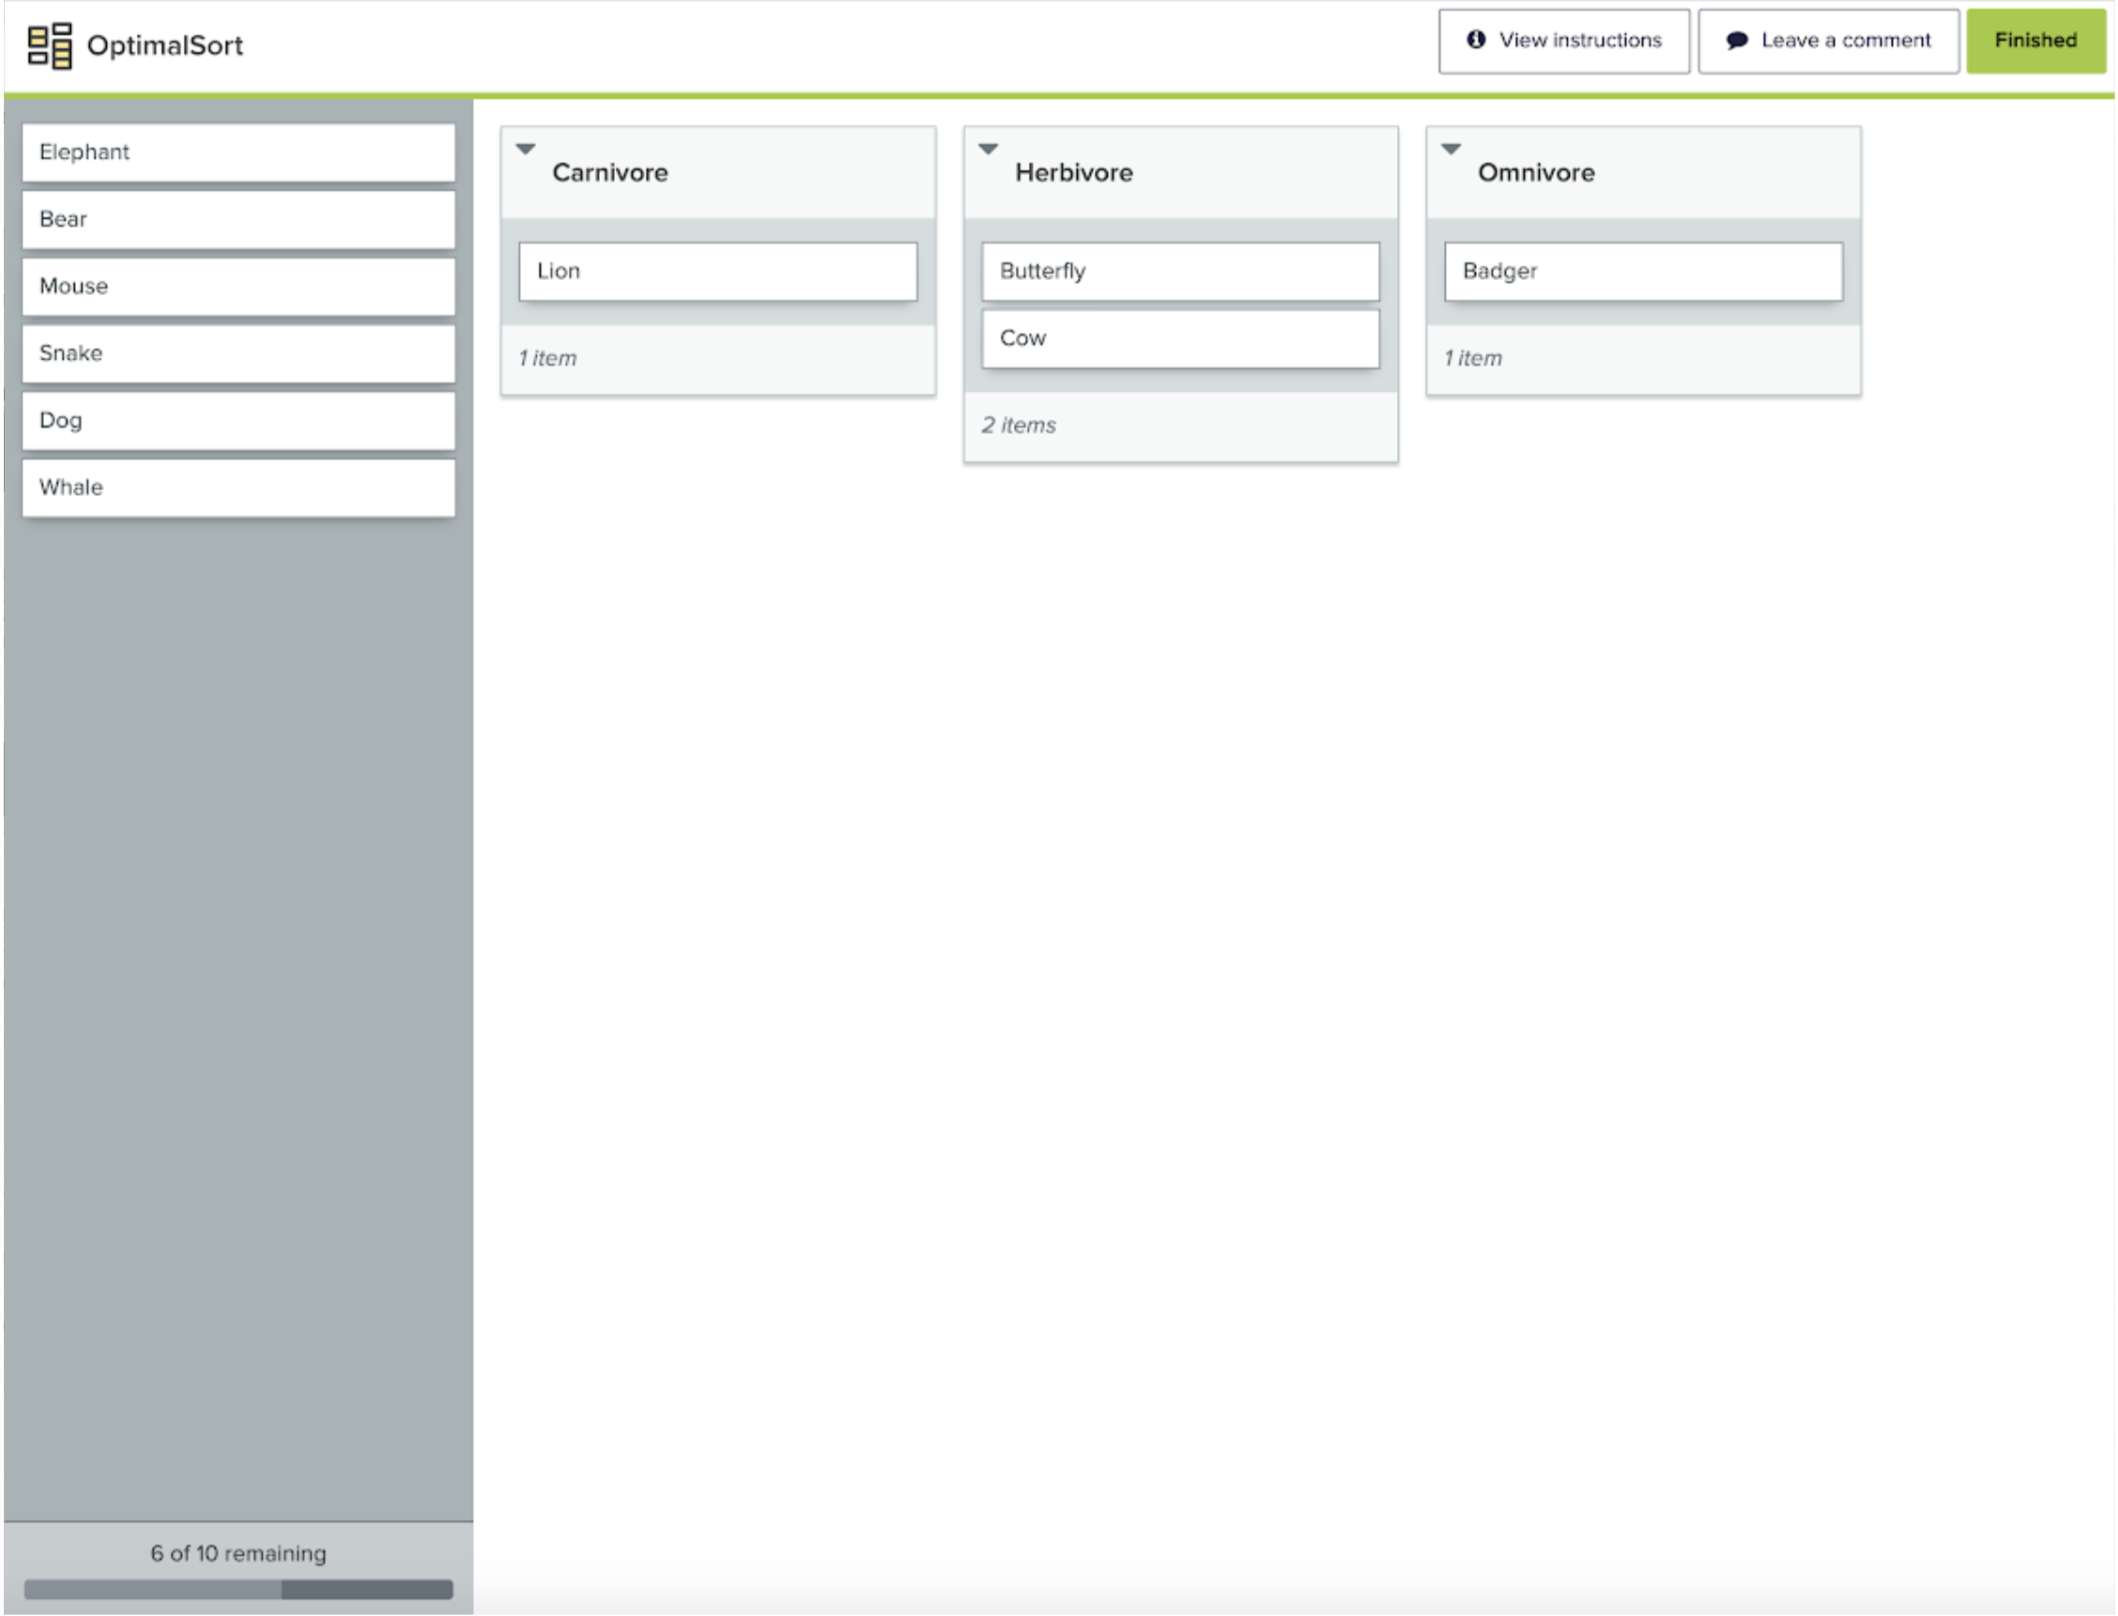
\includegraphics[keepaspectratio,width=\linewidth,height=\halfh]{images/optimalsort-sorting.png}
\caption[OptimalSort Card Sorting] { This is a screenshot during the online card
sorting process in OptimalSort.
\imgcredit{Screenshot was captured by Markus Stradner using
\textcite{OptimalSort} on Safari 14.0.1, 28.11.2020.} }
\label{fig:OptimalSort2}
\end{figure}

After selecting the first item from the list and dragging it to the grouping area a new category is 
created at the open card sorting. At the closed card sorting the categories are fixed permanently. 

In the bottom of each group a helpful counter of the items of the group is displayed. Also for the 
remaining cards a counter is shown in the bottom left corner. In the top right corner there are three 
options available during the study: view the instructions again, leave a comment and finish the 
study. 

After assigning all cards and finishing the the study the thank you message pop up and you are 
done. 


\section{Analytics}
OptimalSort offers a large variety of analysis tools. Beside an overview of the card and
categories section it also offers a standardization grid, similarity matrix, dendrogram, participant-
centric matrix and 3D cluster view. 

\begin{figure}[h] 
\centering
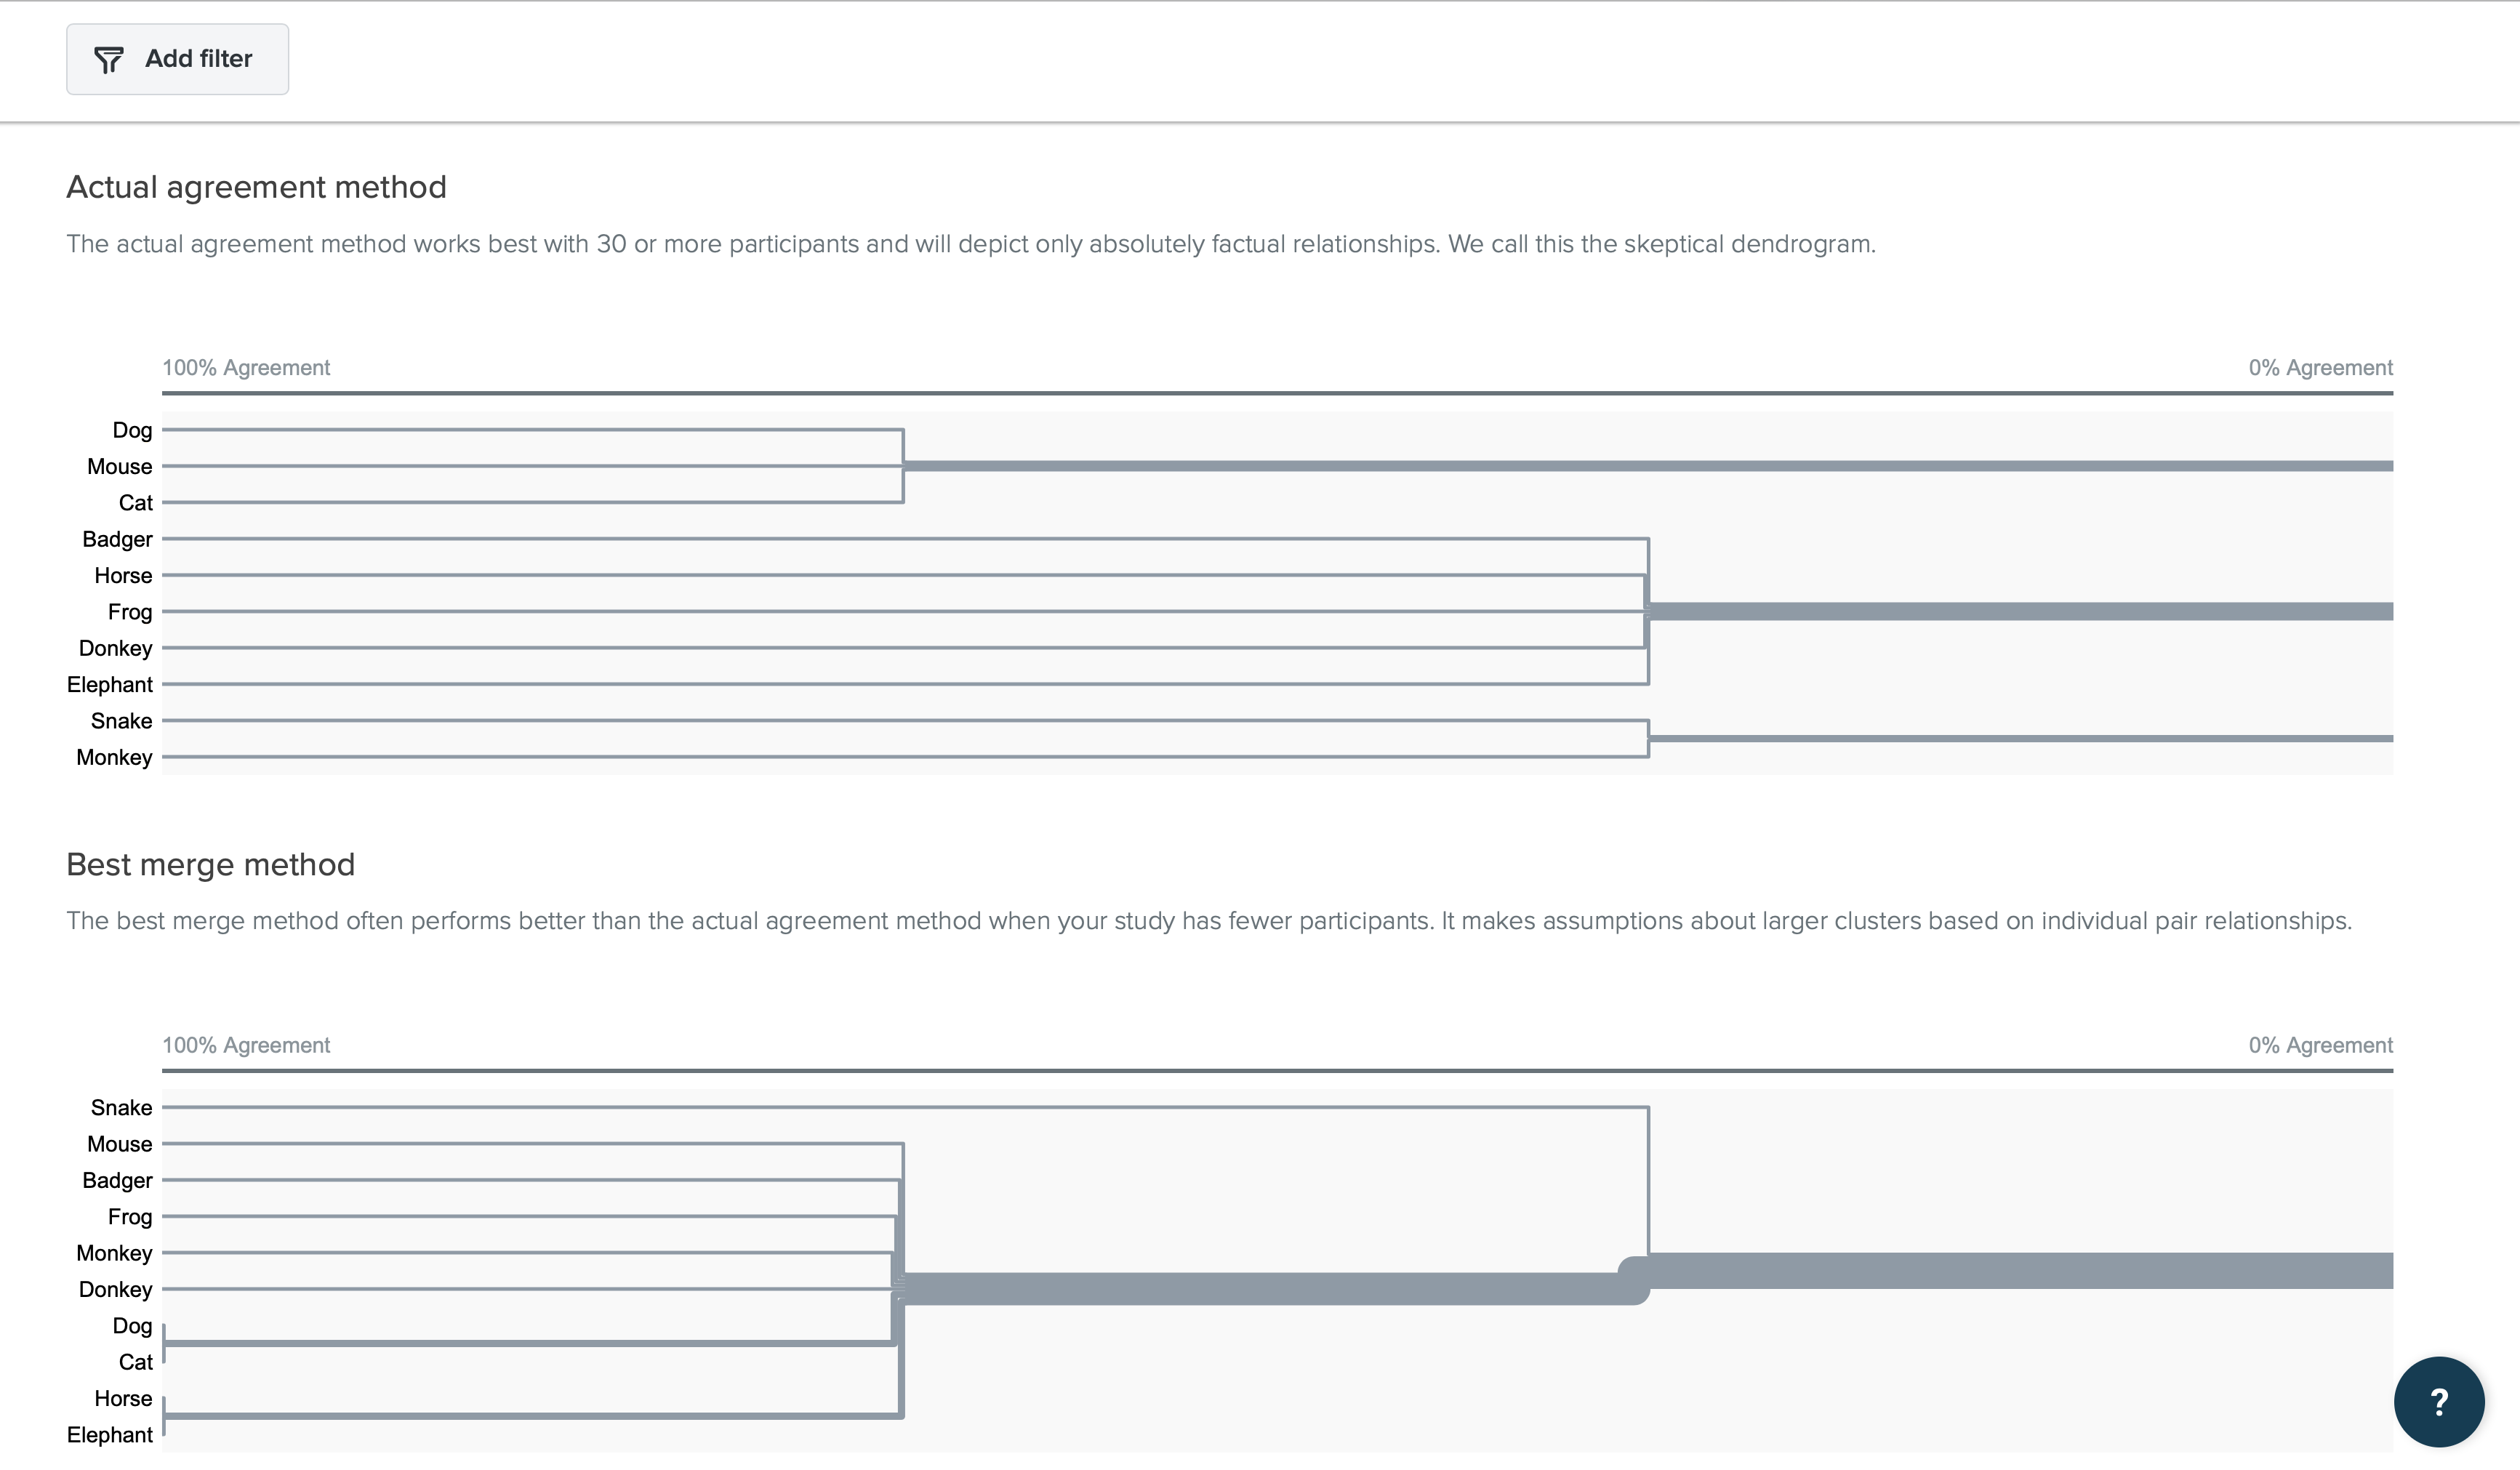
\includegraphics[keepaspectratio,width=\linewidth,height=\halfh]{images/optimalsort-analysis1.png}
\caption[OptimalSort Analysis - Dendrogram] { This screenshot shows a
dendrogram used for analytics.
\imgcredit{Screenshot was captured by Markus Stradner using
\textcite{OptimalSort} on Safari 14.0.1, 28.11.2020.} }
\label{fig:OptimalSort1}
\end{figure}

You can also share the results of the study with other people be creating a link of the desired 
analysis method.

If you would like to save the data also in your local storage, OptimalSort offers an export for the 
following data: 

\begin{itemize}
    \item Raw data (.xlsx)     
    \item Participants data (.xlsx)
    \item SynCaps data (.txt)
    \item Standardized data (.xlsx)
    \item Similarity matrix (.csv)
    \item Standardization grid (.csv)
\end{itemize}


\begin{figure}[t] 
\centering
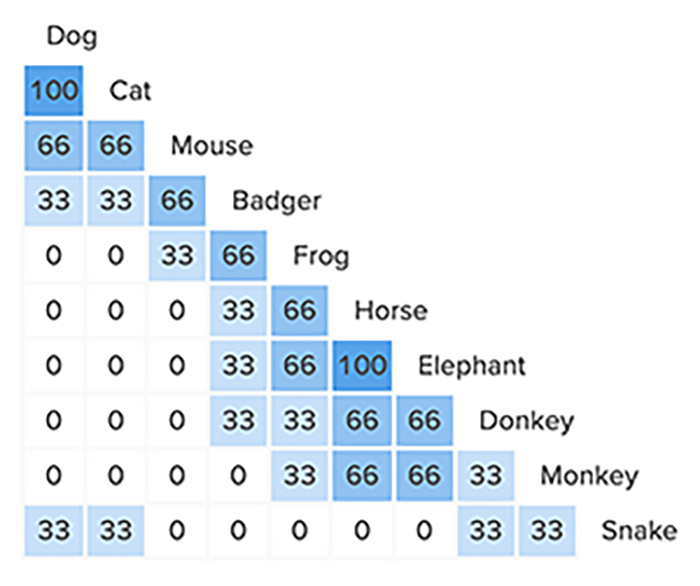
\includegraphics[width=150px]{images/optimalsort-analysis2.png}
\caption[OptimalSort Analysis - Similarity Matrix] { This screenshot shows a
similartiy matrix used for analytics.
\imgcredit{Screenshot was captured by Markus Stradner using
\textcite{OptimalSort} on Safari 14.0.1, 28.11.2020.} }
\label{fig:OptimalSort1}
\end{figure}


\section{Summary \& Ratings}
To sum up OptimalSort you have to mention the nice dashboard with studies, demos, instructions, 10-
step-tutorial and the resource center. Importing and exporting data is also very simple and 
convenient. All the analysis tools are really cool and helpful and are shown in nice charts, tables and 
diagrams. Setting up the study and also participation is very intuitiv and easy to handle.
The disadvantages were only that you need an account and that there is a paywall to get all features. 
A detailed summary of features can be viewed in Table~\ref{tab:features-OptimalSort}.

\begin{table}[h]
\centering
\begin{tabularx}
{\linewidth}{|l|X|}
\hline \textbf{Feature/Characteristic} & \textbf{Availability in OptimalSort} \\ 
\hline Card Sorting & Open, closed and hybrid. \\ 
\hline Card Limit & Free version: 50, paid version: unlimited \\
\hline Participant Limit & Free version: 10, paid version: unlimited \\
\hline Analytics & Overview of cards/categories, standardization grid, similarity matrix, dendrogram, participant-centric matrix, 3D cluster view. \\ 
\hline Documentation & Demos, tutorials, webinars, instructions during card sorting. \\
\hline Business Model & Free version (imited cards, participants and features) and paid version (\$166 per month) with all features. \\
\hline Import formats & provided spreadsheet for cards and categories, pre-defined editable welcome and thank you messages. \\ 
\hline Export formats & .xlsx, .txt, .csv \\ 
\hline Sub-Categories & No. \\ 
\hline Playback of user-sessions & No. \\ 
\hline Data preparation & Only by hand through export files. \\ 
\hline
\end{tabularx} 
\caption[Feature summary of OptimalSort] 
{ 
This table summarizes all the features and characteristics of OptimalSort
to provide an easy to read overview.
}
\label{tab:features-OptimalSort}
\end{table}


For a quick overview we agreed on four ratings for the tool. The ratings can be
found in Table~\ref{tab:rating-OptimalSort} and range from 0-5.

\begin{table}[h] 
\centering 
\begin{tabularx}{\linewidth}{|X|X|X|X|X|}
\hline
Simplicity & Documentation & Features & Business Model & Average \\ 
\hline 
4 & 5 & 5 & 3 & 4.25 \\ 
\hline 
\end{tabularx} 
\caption[Ratings for OptimalSort] {
Ratings for OptimalSort including the average rating.
} 
\label{tab:rating-OptimalSort}
\end{table}






